\documentclass{article}
\usepackage{tikz}
\usetikzlibrary{intersections,shapes.arrows}

\newcommand\Dist[1]{\phantom{\rule{#1}{4pt}}}

\begin{document}
	
	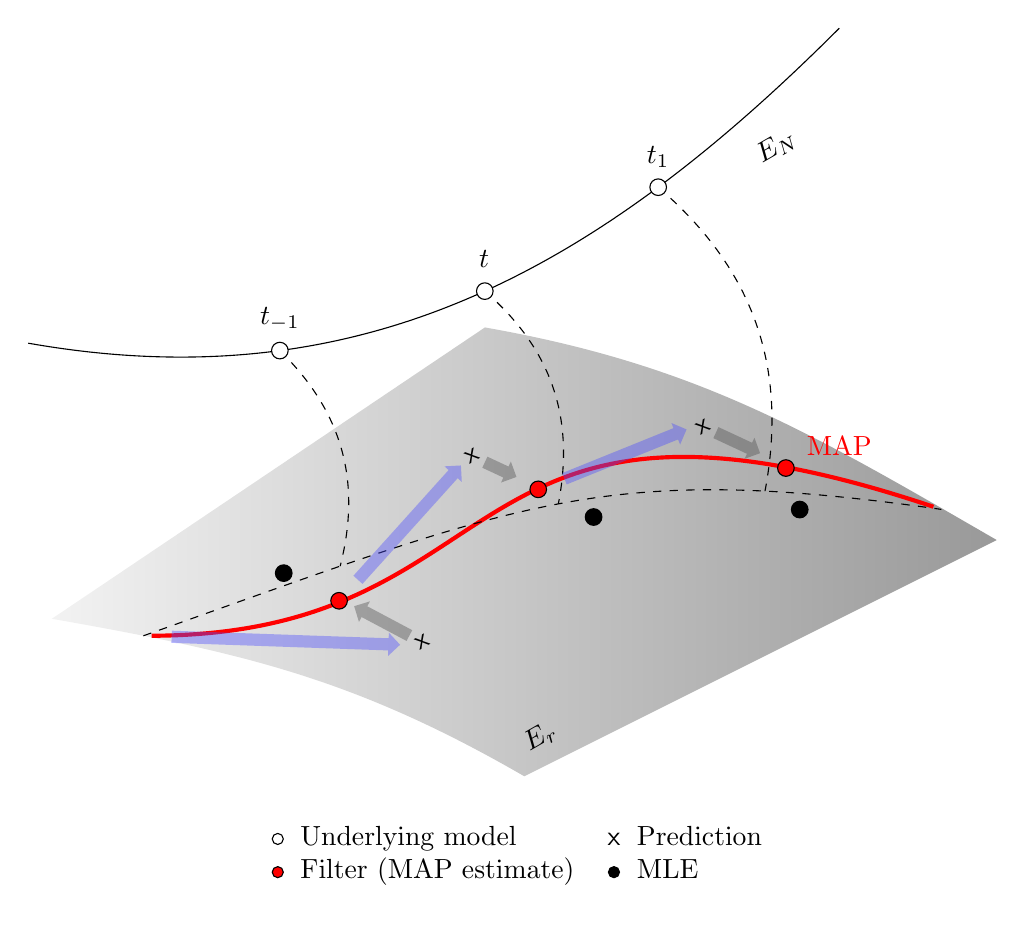
\begin{tikzpicture}
		
		% the bottom left border of the surface
		\path[name path=border1] (0,0) to[out=-10,in=150] (6,-2);
		% the upper right border of the surface
		\path[name path=border2] (12,1) to[out=150,in=-10] (5.5,3.2);
		% a path for a line crossing both borders
		\path[name path=redline] (0,-0.4) -- (12,1.5);
		% intersections between the borders and the lines
		\path[name intersections={of=border1 and redline,by={a}}];
		\path[name intersections={of=border2 and redline,by={b}}];
		
		% we draw the surface
		\shade[left color=gray!10,right color=gray!80] 
		(0,0) to[out=-10,in=150] (6,-2) -- (12,1) to[out=150,in=-10] (5.5,3.7) -- cycle;
		% we draw the red line
		\draw[red,line width=1.5pt,shorten >= 3pt,shorten <= 3pt] 
		(a) .. controls (6,-0.2) and (5,3.5) ..
		coordinate[pos=0.22] (cux1) 
		coordinate[pos=0.57] (cux2) 
		coordinate[pos=0.88] (cux3) (b);
		% we draw the curved black line on top
		\draw (-0.3,3.5) to[out=-10,in=225] 
		coordinate[pos=0.27] (aux1) 
		coordinate[pos=0.52] (aux2) 
		coordinate[pos=0.75] (aux3) (10,7.5);
		% we draw the dashed line on the surface
		\draw[dashed] (a) .. controls (6,1.5) and (7,2) .. 
		coordinate[pos=0.2] (bux1) 
		coordinate[pos=0.5] (bux2) 
		coordinate[pos=0.8] (bux3) (b);
		
		% we draw the dashed lines from the curved line on top to the 
		% dashed line on the surface
		\foreach \coor in {1,2,3}
		\draw[dashed] (aux\coor)to[bend left] (bux\coor);
		% we draw the markers on the top line and place the labels
		\foreach \coor/\subs in {1/-1,2/,3/1}
		{
			\draw[fill=white] (aux\coor) circle (3pt);
			\node[label=above:$t_{\subs}$] at (aux\coor) {};
		}
		% we draw the filled red circles on the red line
		\foreach \coor in {1,2,3}
		\draw[fill=red] (cux\coor) circle (3pt);
		% we draw the filled black circles near the red line
		\draw[fill] ([xshift=-20pt,yshift=10pt]cux1) circle (3pt);
		\draw[fill] ([xshift=20pt,yshift=-10pt]cux2) circle (3pt);
		\draw[fill] ([xshift=5pt,yshift=-15pt]cux3) circle (3pt);
		
		%  we place the "x" labels
		\node (dux1) [xshift=30pt,yshift=-15pt,font=\sffamily,rotate=30] at (cux1) {x};
		\node (dux2) [xshift=-24pt,yshift=12pt,font=\sffamily,rotate=30] at (cux2) {x};
		\node (dux3) [xshift=-30pt,yshift=15pt,font=\sffamily,rotate=30] at (cux3) {x};
		
		% we draw the blue and gray arrows
		\begin{scope}[
			every node/.style={
				inner sep=0pt,
				opacity=0.4,
				single arrow,
				draw=none,
				single arrow head extend=2pt}
			]
			\node[fill=black!70,anchor=west,rotate=152,xshift=5pt] at (dux1) 
			{\Dist{20pt}};
			\node[fill=black!70,anchor=west,rotate=-25,xshift=5pt] at (dux2) 
			{\Dist{10pt}};
			\node[fill=black!70,anchor=west,rotate=-25,xshift=5pt] at (dux3) 
			{\Dist{15pt}};
			
			\node[fill=blue!70,anchor=west,rotate=-2,xshift=10pt] at (a) 
			{\Dist{80pt}};
			\node[fill=blue!70,anchor=west,rotate=48,xshift=10pt] at (cux1) 
			{\Dist{53pt}};
			\node[fill=blue!70,anchor=west,rotate=22,xshift=10pt] at (cux2) 
			{\Dist{45pt}};
		\end{scope}
		
		% we add some labels
		\node[rotate=30] at (6.2,-1.5) {$E_r$};
		\node[rotate=30] at (9.2,6) {$E_N$};
		\node[font=\color{red}] at (10,2.2) {MAP};
		
		\node at ([yshift=-1cm]current bounding box.south) {
			\setlength\tabcolsep{3pt}
			\begin{tabular}{@{}cl@{\hspace{12pt}}cl@{}}
				\tikz\draw (0,0) circle (2pt); & Underlying model & \sffamily x & Prediction \\ 
				\tikz\draw[fill=red] (0,0) circle (2pt); & Filter (MAP estimate) 
				& \tikz\draw[fill] (0,0) circle (2pt); & MLE
			\end{tabular}
		};
	\end{tikzpicture}

\end{document}